\chapter{质点运动学}\label{ch:b1:point-kinematics}

过山车车厢以 \qty{90}{km/h} 的\omterm{def:b1:point-kinematics:velocity}{速度}驶入环路，
爬升时逐渐减速，在顶点停留片刻，随即俯冲而出；
乘客在最低点时被紧紧压在座椅上，
在最高点时几近失重。描述这段运动——车厢在何处、
运动得多快、\omterm{def:b1:point-kinematics:velocity}{速度}如何转动与变化——属于运动学，
而它所需的工具远不止直路上的 $x$、$y$、$z$：凡涉及转动处须用\omterm{def:b1:point-kinematics:cylindrical}{极坐标}，
还需一个随车厢一同运动的\omterm{def:b1:point-kinematics:frame}{参考系}。
本章建立这些工具，并在每种坐标下证明\omterm{def:b1:point-kinematics:velocity}{速度}与\omterm{def:b1:point-kinematics:velocity}{加速度}的公式，
再将其应用于此后各章都会用到的运动：\omterm{cor:b1:point-kinematics:circular}{圆周运动}、
\omterm{prop:b1:point-kinematics:helix}{螺旋运动}、\omterm{prop:b1:point-kinematics:harmonic}{简谐运动}，
以及沿任意曲线的运动。

\section{位置、速度与加速度}

\begin{definition}[参考系；位置；轨迹]\label{def:b1:point-kinematics:frame}
\index{参考系}\index{位置矢量}\index{轨迹}\index{质点}
\emph{参考系}是取作静止的刚体（
如实验室、地球、火车），并配有一只时钟。\emph{质点}
$M$——大小与所研究运动无关的物体，
在每一时刻由其\emph{位置矢量}
$\vect{OM}(t)$ 确定，原点 $O$ 与参考系固连；
$M$ 所描出的曲线称为它的\emph{轨迹}。
运动总是\emph{相对于参考系}而言的：
同一位乘客，在火车上是静止的，在车站里却是运动的。
\end{definition}

\begin{definition}[速度与加速度]\label{def:b1:point-kinematics:velocity}
\index{速度}\index{加速度}
在\omterm{def:b1:point-kinematics:frame}{参考系}中，$M$ 的\emph{速度}与\emph{加速度}分别为
\[
\vect v = \frac{\dd\vect{OM}}{\dd t}, \qquad
\vect a = \frac{\dd\vect v}{\dd t} = \frac{\dd^2\vect{OM}}{\dd t^2},
\]
矢量函数的导数：矢量的导数是通过对其分量求导得到的，
所取的基底须是
\emph{固连于\omterm{def:b1:point-kinematics:frame}{参考系}}的。速度沿\omterm{def:b1:point-kinematics:frame}{轨迹}切线，
指向运动方向；其模 $v$ 即\emph{速率}。单位：
\unit{m/s}, \unit{m/s^2}.
\end{definition}

\begin{proposition}[直角坐标]\label{prop:b1:point-kinematics:cartesian}
\index{直角坐标}
取固定的正交归一基 $(\vect e_x, \vect e_y, \vect e_z)$，并记
$\vect{OM} = x\,\vect e_x + y\,\vect e_y + z\,\vect e_z$,
\[
\vect v = \dot x\,\vect e_x + \dot y\,\vect e_y + \dot z\,\vect e_z, \qquad
\vect a = \ddot x\,\vect e_x + \ddot y\,\vect e_y + \ddot z\,\vect e_z,
\]
其中点号表示 $\dd/\dd t$。
\end{proposition}

\begin{proof}
基矢量为常矢量，只有分量随时间变化。
\end{proof}

\begin{example}[抛体]\label{ex:b1:point-kinematics:projectile}
自 $O$ 以速率 $v_0$、与水平面成 $\alpha$ 角斜向上抛出，
小球的坐标（动力学内容留待下一章）为
$x = v_0\cos\alpha\,t$，$z = v_0\sin\alpha\,t - \tfrac12 gt^2$。于是
$\vect v = v_0\cos\alpha\,\vect e_x + (v_0\sin\alpha - gt)\vect e_z$,
$\vect a = -g\vect e_z$：\omterm{def:b1:point-kinematics:velocity}{加速度}恒定，而
\omterm{def:b1:point-kinematics:velocity}{速度}方向不断改变；在顶点（$\dot z = 0$，$t = v_0\sin\alpha/g$）处
\omterm{def:b1:point-kinematics:velocity}{速度}水平，\omterm{def:b1:point-kinematics:velocity}{加速度}与之垂直。
消去 $t$ 得 $z = x\tan\alpha - gx^2/(2v_0^2\cos^2\alpha)$，为一条
抛物线。
\end{example}

\begin{omfigure}
\begin{tikzpicture}[font=\small, x=1cm, y=1cm]
  \draw[-Stealth] (0,0) -- (6.8,0) node[right] {$x$};
  \draw[-Stealth] (0,0) -- (0,3.6) node[above] {$z$};
  \node[below left] at (0,0) {$O$};
  \draw[omDef, thick, domain=0:6, samples=80] plot (\x, {2.2*\x - 0.3667*\x*\x});
  % point at x=1.5: z=2.2*1.5-0.3667*2.25=3.3-0.825=2.475 ; slope = 2.2 - 0.7333*1.5 = 1.1
  \fill[omThm] (1.5,2.475) circle (1.6pt); \node[above left] at (1.5,2.475) {$M$};
  \draw[-Stealth, omThm, thick] (1.5,2.475) -- ++(1.0,1.1) node[above right] {$\vect v$};
  \draw[-Stealth, omProp, thick] (1.5,2.475) -- ++(0,-1.2) node[right] {$\vect a = \vect g$};
  \draw[-Stealth, omExo] (0,0) -- (1.5,2.475); \node[omExo, left] at (0.72,1.45) {$\vect{OM}$};
  % apex at x=3: z=6.6-3.3=3.3
  \fill[omThm] (3,3.3) circle (1.6pt);
  \draw[-Stealth, omThm, thick] (3,3.3) -- ++(1.2,0);
  \draw[-Stealth, omProp, thick] (3,3.3) -- ++(0,-1.2);
\end{tikzpicture}

{\small 抛体的抛物线：\omterm{def:b1:point-kinematics:velocity}{速度}与\omterm{def:b1:point-kinematics:frame}{轨迹}相切，
方向不断改变，\omterm{def:b1:point-kinematics:velocity}{加速度} $\vect g$ 恒定。在顶点
处\omterm{def:b1:point-kinematics:velocity}{速度}与\omterm{def:b1:point-kinematics:velocity}{加速度}相互垂直：速率此刻不变，
而\omterm{def:b1:point-kinematics:velocity}{速度}方向仍在改变。}
\end{omfigure}

\section{柱坐标}

\begin{definition}[柱坐标与基]\label{def:b1:point-kinematics:cylindrical}
\index{柱坐标}\index{极坐标}\index{局部基}
\omterm{def:b1:point-kinematics:frame}{质点} $M$ 的位置由 $r \geq 0$（到 $z$ 轴的距离）、
角 $\theta$（其投影在 $xy$ 平面上，与 $\vect e_x$ 的夹角）、
以及 $z$：$\vect{OM} = r\,\vect e_r + z\,\vect e_z$，其中
\[
\vect e_r = \cos\theta\,\vect e_x + \sin\theta\,\vect e_y, \qquad
\vect e_\theta = -\sin\theta\,\vect e_x + \cos\theta\,\vect e_y,
\]
而 $\vect e_z$ 与 $(\vect e_r, \vect e_\theta,
\vect e_z)$ 构成\emph{局部基}，它正交归一且为右手系，\emph{随 $M$ 一起运动}。
在平面内（$z$ 固定）时，它们即为\emph{极坐标} $(r, \theta)$。
\end{definition}

\begin{lemma}[局部基的导数]\label{lem:b1:point-kinematics:basisderiv}
\[
\frac{\dd\vect e_r}{\dd t} = \dot\theta\,\vect e_\theta, \qquad
\frac{\dd\vect e_\theta}{\dd t} = -\dot\theta\,\vect e_r, \qquad
\frac{\dd\vect e_z}{\dd t} = \vect 0 .
\]
\end{lemma}

\begin{proof}
对各分量求导：$\dd\vect e_r/\dd t = \dot\theta(-\sin\theta\,
\vect e_x + \cos\theta\,\vect e_y) = \dot\theta\vect e_\theta$，且
对 $\vect e_\theta$ 同理。旋转单位矢量的导数
与其垂直，模等于角速率。
\end{proof}

\begin{theorem}[柱坐标中的速度与加速度]\label{thm:b1:point-kinematics:cylindrical}
\[
\vect v = \dot r\,\vect e_r + r\dot\theta\,\vect e_\theta + \dot z\,\vect e_z,
\qquad
\vect a = \big(\ddot r - r\dot\theta^2\big)\vect e_r
+ \big(r\ddot\theta + 2\dot r\dot\theta\big)\vect e_\theta + \ddot z\,\vect e_z .
\]
\end{theorem}

\begin{proof}
对 $\vect{OM} = r\vect e_r + z\vect e_z$ 利用引理求导：
$\vect v = \dot r\vect e_r + r\dot\theta\vect e_\theta + \dot z\vect e_z$.
再次求导：$\ddot r\vect e_r + \dot r\dot\theta\vect e_\theta +
\dot r\dot\theta\vect e_\theta + r\ddot\theta\vect e_\theta - r\dot\theta^2
\vect e_r + \ddot z\vect e_z$，合并同类项。
\end{proof}

\begin{omfigure}
\begin{tikzpicture}[font=\small, x=1cm, y=1cm]
  \draw[-Stealth] (0,0) -- (5.2,0) node[right] {$x$};
  \draw[-Stealth] (0,0) -- (0,3.6) node[above] {$y$};
  \node[below left] at (0,0) {$O$};
  \coordinate (M) at (35:3.4);
  \draw[omExo] (0,0) -- (M); \fill[omThm] (M) circle (1.6pt); \node[below right, xshift=2pt] at (M) {$M$};
  \node[omExo] at (20:1.9) {$r$};
  \draw (0.9,0) arc (0:35:0.9); \node at (17:1.15) {$\theta$};
  \draw[-Stealth, omDef, very thick] (M) -- ++(35:1.1) node[right] {$\vect e_r$};
  \draw[-Stealth, omDef, very thick] (M) -- ++(125:1.0) node[left] {$\vect e_\theta$};
  % trajectory sketch: spiral
  \draw[omThm, thick, domain=5:75, samples=50, variable=\t] plot ({(2.2+0.0343*\t)*cos(\t)},{(2.2+0.0343*\t)*sin(\t)});
  \draw[-Stealth, omThm, thick] (M) -- ++(100:1.6) node[above right] {$\vect v$};
\end{tikzpicture}

{\small \omterm{def:b1:point-kinematics:cylindrical}{极坐标}：\omterm{def:b1:point-kinematics:cylindrical}{局部基} $(\vect e_r, \vect e_\theta)$
随 $M$ 转动；\omterm{def:b1:point-kinematics:velocity}{速度}有径向分量 $\dot r$ 和
横向分量 $r\dot\theta$。此处\omterm{def:b1:point-kinematics:frame}{轨迹}（红色）向外螺旋，
故 $\dot r > 0$，$\vect v$ 向外偏离
圆的切线方向。}
\end{omfigure}

\begin{corollary}[圆周运动]\label{cor:b1:point-kinematics:circular}
\index{圆周运动}\index{向心加速度}\index{角速度}
在半径为 $R$ 的圆上（$r = R$，$z = 0$），取\emph{\omterm{cor:b1:point-kinematics:circular}{角
速度}} $\omega = \dot\theta$：
\[
\vect v = R\omega\,\vect e_\theta, \qquad
\vect a = -R\omega^2\,\vect e_r + R\dot\omega\,\vect e_\theta
= -\frac{v^2}{R}\,\vect e_r + \frac{\dd v}{\dd t}\,\vect e_\theta .
\]
对\emph{匀速}\omterm{cor:b1:point-kinematics:circular}{圆周运动}（$\omega$ 为常数），\omterm{def:b1:point-kinematics:velocity}{加速度}
完全是\emph{向心的}，模为 $v^2/R = R\omega^2$，
尽管速率保持不变。
\end{corollary}

\begin{proof}
在定理中令 $\dot r = \ddot r = 0$；此时 $v = R\omega$。
\end{proof}

\begin{example}[两个圆周运动]\label{ex:b1:point-kinematics:circles}
一辆汽车绕半径为 \qty{20}{m} 的环岛行驶，速率为 \qty{36}{km/h}
（\qty{10}{m/s}）：$a = v^2/R = \qty{5.0}{m/s^2}$，即半个 $g$，方向
指向圆心——轮胎必须提供的力。月球
（$R = \qty{3.84e8}{m}$，$T = \qty{27.3}{d}$）：$\omega = 2\pi/T =
\qty{2.66e-6}{rad/s}$，$a = R\omega^2 = \qty{2.7e-3}{m/s^2}$，
即 $3600$ 分之一个地表 $g$，距地心六十个地球半径——
牛顿所作的比较（见\cref{ch:b1:central-forces}）。
\end{example}

\section{球坐标}

\begin{definition}[球坐标]\label{def:b1:point-kinematics:spherical}
\index{球坐标}
点 $M$ 的位置由其到原点的距离 $r = OM$、\emph{余纬}
$\theta \in [0, \pi]$（$\vect{OM}$ 与 $\vect e_z$ 的夹角）以及
\emph{方位角} $\varphi$（其在 $xy$ 平面上的投影）确定：
$\vect{OM} = r\,\vect e_r$，其中
\[
\vect e_r = \sin\theta\cos\varphi\,\vect e_x + \sin\theta\sin\varphi\,\vect e_y + \cos\theta\,\vect e_z ;
\]
$\vect e_\theta$（与经线相切，指向 $\theta$ 增大的方向）
与 $\vect e_\varphi$（与纬线相切）一起构成局部
正交归一基。在地球上，$\theta$ 为 $90^\circ$ 减去
纬度，$\varphi$ 为经度。
\end{definition}

\begin{proposition}[球坐标中的速度]\label{prop:b1:point-kinematics:sphericalv}
\[
\vect v = \dot r\,\vect e_r + r\dot\theta\,\vect e_\theta + r\sin\theta\,\dot\varphi\,\vect e_\varphi .
\]
\end{proposition}

\begin{proof}
$\dd\vect e_r/\dd t = \dot\theta\,\vect e_\theta + \sin\theta\,\dot\varphi\,
\vect e_\varphi$：第一项为经线面内的转动
（与\omterm{def:b1:point-kinematics:cylindrical}{极坐标}情形相同），第二项是绕 $\vect e_z$ 的转动，角速率为
$\dot\varphi$，作用于到轴距离为
$\sin\theta$ 的矢量。于是 $\vect v = \dd(r\vect e_r)/\dd t$。
本学年不需要\omterm{def:b1:point-kinematics:velocity}{加速度}。
\end{proof}

\begin{omfigure}
\begin{tikzpicture}[font=\small, x=1cm, y=1cm, scale=0.95]
  \draw[-Stealth] (0,0) -- (-2.4,-0.96) node[below left] {$x$};
  \draw[-Stealth] (0,0) -- (4.2,0) node[right] {$y$};
  \draw[-Stealth] (0,0) -- (0,3.6) node[above] {$z$};
  \node[below right] at (0,0) {$O$};
  \coordinate (M) at (1.4,2.4);
  \coordinate (P) at (1.4,-0.3);
  \draw[omExo] (0,0) -- (M); \fill[omThm] (M) circle (1.6pt); \node[above left] at (M) {$M$};
  \draw[dashed] (M) -- (P); \draw[dashed] (0,0) -- (P);
  \node[omExo] at (0.45,1.45) {$r$};
  \draw (0,1.0) arc (90:60:1.0); \node at (0.3,1.25) {$\theta$};
  \draw (-0.74,-0.3) arc (202:348:0.8); \node at (0.15,-1.05) {$\varphi$};
  \draw[-Stealth, omDef, very thick] (M) -- ++(0.45,0.77) node[above] {$\vect e_r$};
  \draw[-Stealth, omDef, very thick] (M) -- ++(0.77,-0.45) node[right] {$\vect e_\theta$};
  \draw[-Stealth, omDef, very thick] (M) -- ++(0.84,0.33) node[right] {$\vect e_\varphi$};
\end{tikzpicture}

{\small \omterm{def:b1:point-kinematics:spherical}{球坐标} $(r, \theta, \varphi)$ 及其\omterm{def:b1:point-kinematics:cylindrical}{局部
基}：$\vect e_r$ 为径向，$\vect e_\theta$ 沿子午线（
在地球仪上指向南），$\vect e_\varphi$ 沿纬线（
指向东）。}
\end{omfigure}

\section{弗勒内标架}

\begin{definition}[曲线坐标；弗勒内基]\label{def:b1:point-kinematics:frenet}
\index{曲线坐标}\index{弗勒内基}\index{曲率半径}
沿\omterm{def:b1:point-kinematics:frame}{轨迹}，\emph{曲线坐标} $s(t)$ 为自参考点起算的
弧长（按代数值计）；$v = \dot s$。在
$M$ 处，单位切向量 $\vect T = \dd\vect{OM}/\dd s$ 沿
$s$ 增大的方向；\emph{曲率半径} $\rho > 0$ 与单位
法向量 $\vect N$ 指向凹侧（即曲率中心所在一侧），
由下式定义：
\[
\frac{\dd\vect T}{\dd s} = \frac{1}{\rho}\,\vect N .
\]
$(\vect T, \vect N)$ 称为\emph{弗勒内基}；$\rho = \infty$ 对应
直线，$\rho = R$ 对应半径为 $R$ 的圆。
\end{definition}

\begin{theorem}[弗勒内基下的加速度]\label{thm:b1:point-kinematics:frenet}
\index{切向加速度}\index{法向加速度}
\[
\vect v = v\,\vect T, \qquad
\vect a = \frac{\dd v}{\dd t}\,\vect T + \frac{v^2}{\rho}\,\vect N .
\]
\emph{切向}分量 $\dd v/\dd t$ 刻画速率变化的快慢；
\emph{法向}分量 $v^2/\rho$ 总指向曲率中心，刻画
方向转动的快慢。运动是匀速的，当且仅当 $\vect a \perp \vect v$；
运动为直线运动，当且仅当
$\vect a \parallel \vect v$。
\end{theorem}

\begin{proof}
$\vect v = (\dd\vect{OM}/\dd s)(\dd s/\dd t) = v\vect T$。于是 $\vect a =
\dot v\vect T + v\,\dd\vect T/\dd t = \dot v\vect T + v(\dd\vect T/\dd s)\dot s
= \dot v\vect T + (v^2/\rho)\vect N$。$\dd\vect T/\dd s \perp \vect T$
可由 $\vect T\cdot\vect T = 1$ 求导得出。
\end{proof}

\begin{omfigure}
\begin{tikzpicture}[font=\small, x=1cm, y=1cm]
  \draw[omDef, thick, domain=-2.6:3.2, samples=80] plot (\x, {0.22*\x*\x - 0.05*\x*\x*\x});
  % point at x=1: y=0.17 ; slope = 0.44-0.15=0.29 -> T direction angle 16.2 deg
  \coordinate (M) at (1,0.17);
  \fill[omThm] (M) circle (1.6pt); \node[below right] at (M) {$M$};
  \draw[-Stealth, omThm, very thick] (M) -- ++(16.2:1.2) node[right] {$\vect T$};
  \draw[-Stealth, omThm, very thick] (M) -- ++(106.2:1.2) node[above] {$\vect N$};
  % center of curvature: curvature kappa = y''/(1+y'^2)^{3/2}: y''=0.44-0.3=0.14 ; (1+0.0841)^1.5=1.129 -> kappa=0.124 -> rho=8.06 (too big) ; draw just arrow to C off-figure shortened
  \draw[dashed, omExo] (M) -- ++(106.2:3.0) node[above] {指向 $C$，距离为 $\rho$};
  \draw[-Stealth, omProp, thick] (M) -- ++(16.2:0.8) ++(0,0) -- ++(106.2:1.0);
  \draw[-Stealth, omProp, very thick] (M) -- ($(M)+(16.2:0.8)+(106.2:1.0)$) node[above right] {$\vect a$};
  \node[omProp, font=\footnotesize] at ($(M)+(16.2:0.95)+(0,-0.25)$) {$\dot v$};
  \node[omProp, font=\footnotesize] at ($(M)+(16.2:0.8)+(106.2:0.5)+(0.25,0)$) {$v^2/\rho$};
\end{tikzpicture}

{\small 曲线上一点处的\omterm{def:b1:point-kinematics:frenet}{弗勒内基}：$\vect T$ 沿
运动方向，$\vect N$ 指向曲率中心 $C$。\omterm{def:b1:point-kinematics:velocity}{加速度}
分解为切向部分 $\dot v\vect T$（加速或减速）
与法向部分 $(v^2/\rho)\vect N$（转弯）。}
\end{omfigure}

\begin{example}[弯道减速]\label{ex:b1:point-kinematics:bend}
一辆汽车以 \qty{90}{km/h}（\qty{25}{m/s}）的速率行驶于半径为
\qty{100}{m} 的弯道中，以 \qty{2.0}{m/s^2} 的\omterm{def:b1:point-kinematics:velocity}{加速度}刹车：$a_T = \qty{-2.0}{m/s^2}$，$a_N = 625/100 =
\qty{6.25}{m/s^2}$，$a = \sqrt{4 + 39} = \qty{6.6}{m/s^2}$。法向
分量占主导：弯道首先是转弯问题，而轮胎的抓地力
（下一章）限制了 $\sqrt{a_T^2 + a_N^2}$，这就是为何要
\emph{在入弯之前}刹车。
\end{example}

\section{典型运动}

\begin{proposition}[匀变速直线运动]\label{prop:b1:point-kinematics:uarm}
\index{匀变速运动}
沿一条坐标轴，$\ddot x = a$ 为常量，初始位置为 $x_0$，初\omterm{def:b1:point-kinematics:velocity}{速度}为 $v_0$：
$v = v_0 + at$，$x = x_0 + v_0t + \tfrac12 at^2$，且
$v^2 - v_0^2 = 2a(x - x_0)$。
\end{proposition}

\begin{proof}
两次积分；由前两式消去 $t$。
\end{proof}

\begin{proposition}[螺旋运动]\label{prop:b1:point-kinematics:helix}
\index{螺旋运动}
$r = R$，$\theta = \omega t$，$z = v_zt$（$R$、$\omega$、$v_z$ 为常量）：
速率 $v = \sqrt{R^2\omega^2 + v_z^2}$ 为常量，\omterm{def:b1:point-kinematics:velocity}{加速度}
$\vect a = -R\omega^2\vect e_r$ 为模长恒定的\omterm{cor:b1:point-kinematics:circular}{向心加速度}，且
\omterm{def:b1:point-kinematics:frenet}{曲率半径}为 $\rho = v^2/a = R(1 + v_z^2/R^2\omega^2) > R$。
\end{proposition}

\begin{proof}
由\cref{thm:b1:point-kinematics:cylindrical}，取 $\dot r = 0$，
$\ddot\theta = 0$，$\ddot z = 0$；匀速运动，故 $\vect a$ 纯为
法向的，且 $v^2/\rho = R\omega^2$。
\end{proof}

\begin{proposition}[简谐运动]\label{prop:b1:point-kinematics:harmonic}
\index{简谐运动}
$x = A\cos(\omega t + \varphi)$：$\dot x = -A\omega\sin(\omega t + \varphi)$，
$\ddot x = -\omega^2 x$。\omterm{def:b1:point-kinematics:velocity}{速度}相对位置超前四分之一
周期，\omterm{def:b1:point-kinematics:velocity}{加速度}与位置反向；$v_{\max} =
A\omega$，$a_{\max} = A\omega^2$。它是
半径为 $A$、\omterm{cor:b1:point-kinematics:circular}{角速度}为 $\omega$ 的匀速\omterm{cor:b1:point-kinematics:circular}{圆周运动}在一条直径上的投影。
\end{proposition}

\begin{proof}
求导；对于投影，取 $x = A\cos\theta$，其中 $\theta =
\omega t + \varphi$。
\end{proof}

\begin{method}[选取坐标]\label{met:b1:point-kinematics:choose}
\begin{itemize}
  \item 直线运动或抛物线运动，\omterm{def:b1:point-kinematics:velocity}{加速度}恒定：
        \omterm{prop:b1:point-kinematics:cartesian}{直角坐标}。
  \item 绕某一轴或某一点的运动（圆周、螺旋线、轨道、
        转盘）：用\omterm{def:b1:point-kinematics:cylindrical}{柱坐标}或\omterm{def:b1:point-kinematics:cylindrical}{极坐标}；基矢随运动而变，故应使用
        \cref{thm:b1:point-kinematics:cylindrical}，切勿
        直接对分量求导。
  \item 给定曲线（轨道、弯道、环线）且速率规律已知时：
        用弗勒内标架，它把“快慢”与“方向”分开。
\end{itemize}
无论怎样选取，$\vect v$ 与 $\vect a$ 都是依赖\omterm{def:b1:point-kinematics:frame}{参考系}的
矢量，只有写明\omterm{def:b1:point-kinematics:frame}{参考系}，结果才完整。
\end{method}

\section{练习}

\begin{exercise}[$\star$]\label{exo:b1:point-kinematics:1}
一辆汽车从静止出发，$x(t) = 2.0\,t^2$（\omterm{def:b1:units-dimensions:si}{国际单位制}）。求\omterm{def:b1:point-kinematics:velocity}{速度}与
\omterm{def:b1:point-kinematics:velocity}{加速度}（$t = \qty{3.0}{s}$ 时）；求前
\qty{5}{s} 内经过的距离，以及达到 \qty{100}{km/h} 所需的时间。
\end{exercise}

\begin{exercise}[$\star$]\label{exo:b1:point-kinematics:2}
一\omterm{def:b1:point-kinematics:frame}{质点}在平面内运动，$r = \qty{2.0}{m}$，$\theta = 3.0\,t$
（弧度，\omterm{def:b1:units-dimensions:si}{国际单位制}）。求\omterm{def:b1:point-kinematics:cylindrical}{极坐标}基下的 $\vect v$ 与 $\vect a$、
它们的模，并说明运动的性质。
\end{exercise}

\begin{exercise}[$\star$]\label{exo:b1:point-kinematics:3}
赤道上的一点（$R = \qty{6.37e6}{m}$，恒星日
\qty{86164}{s}）：求其在地心\omterm{def:b1:point-kinematics:frame}{参考系}中的速率与\omterm{def:b1:point-kinematics:velocity}{加速度}。
将该\omterm{def:b1:point-kinematics:velocity}{加速度}与 $g$ 作比较。
\end{exercise}

\begin{exercise}[$\star$]\label{exo:b1:point-kinematics:4}
一球以 $v_0 = \qty{12}{m/s}$、$\alpha = 40^\circ$ 抛出；其坐标
与\cref{ex:b1:point-kinematics:projectile}中的一致。
求到达最高点的时间、最大高度、射程，以及
落地时的\omterm{def:b1:point-kinematics:velocity}{速度}。
\end{exercise}

\begin{exercise}[$\star\star$]\label{exo:b1:point-kinematics:5}
一名骑车人以 \qty{10}{m/s} 的速率进入半径为 \qty{25}{m} 的弯道，
并以 \qty{1.0}{m/s^2} 的\omterm{def:b1:point-kinematics:velocity}{加速度}加速。求\omterm{def:b1:point-kinematics:frenet}{弗勒内基}下的 $\vect a$ 与
其模；若在同一弯道上以相同\omterm{def:b1:point-kinematics:velocity}{加速度}再运动 \qty{5}{s}，结果如何？
\end{exercise}

\begin{exercise}[$\star\star$]\label{exo:b1:point-kinematics:6}
一\omterm{def:b1:point-kinematics:frame}{质点}沿螺线 $r = b\theta$、$\theta = \omega t$ 运动（$b$、
$\omega$ 为常量）。求\omterm{def:b1:point-kinematics:cylindrical}{极坐标}基下的 $\vect v$、速率与 $\vect a$。
$2\dot r\dot\theta$ 项从何而来？
\end{exercise}

\begin{exercise}[$\star\star$]\label{exo:b1:point-kinematics:7}
螺旋线：$R = \qty{2.0}{m}$，$\omega = \qty{1.0}{rad/s}$，$v_z = \qty{0.50}{m/s}$。
求速率、\omterm{def:b1:point-kinematics:velocity}{加速度}、螺距与\omterm{def:b1:point-kinematics:frenet}{曲率半径}。
\end{exercise}

\begin{exercise}[$\star\star$]\label{exo:b1:point-kinematics:8}
一活塞的运动规律为 $x = 0.10\cos(10t)$（\omterm{def:b1:units-dimensions:si}{国际单位制}）。求 $v_{\max}$、$a_{\max}$、
$x$、$v$、$a$ 之间的\omterm{def:b1:wave-propagation:signal}{相位}关系，以及
$\abs v$ 与 $\abs a$ 取最大值时所在的位置。
\end{exercise}

\begin{exercise}[$\star\star$]\label{exo:b1:point-kinematics:9}
从 $\vect e_r = \cos\theta\,\vect e_x + \sin\theta\,\vect e_y$ 出发，
推导 $\dd\vect e_r/\dd t$ 与 $\dd\vect e_\theta/\dd t$，然后得到
\cref{thm:b1:point-kinematics:cylindrical}中的\omterm{def:b1:point-kinematics:cylindrical}{极坐标}\omterm{def:b1:point-kinematics:velocity}{速度}与\omterm{def:b1:point-kinematics:velocity}{加速度}。
\end{exercise}

\begin{exercise}[$\star\star\star$]\label{exo:b1:point-kinematics:10}
对于\cref{ex:b1:point-kinematics:projectile}中的抛体，求
其\omterm{def:b1:point-kinematics:frame}{轨迹}在最高点与发射点处的\omterm{def:b1:point-kinematics:frenet}{曲率半径}，
（利用 $\vect g$ 的法向分量）。哪一处更小？
为什么？
\end{exercise}

\begin{exercise}[$\star\star\star$]\label{exo:b1:point-kinematics:11}
半径为 $R$ 的车轮以速率 $v$ 作无滑动滚动；其轮缘上一点的坐标为
$x = vt - R\sin(vt/R)$，$y = R - R\cos(vt/R)$
（摆线）。求其\omterm{def:b1:point-kinematics:velocity}{速度}与\omterm{def:b1:point-kinematics:velocity}{加速度}；证明该点触地时
\omterm{def:b1:point-kinematics:velocity}{速度}为零，\omterm{def:b1:point-kinematics:velocity}{加速度}为
$v^2/R$，方向竖直向上；求其在最高处的速率。
\end{exercise}

\begin{exercise}[$\star\star\star$]\label{exo:b1:point-kinematics:12}
一人沿转盘的半径向外行走，转盘以恒定的
$\omega$ 转动，人相对转盘以恒定速率 $u$ 运动：
$r = ut$，$\theta = \omega t$。求\omterm{def:b1:point-kinematics:cylindrical}{极坐标}基下的 $\vect a$，
指出其中的两项，并计算 $u = \qty{1.0}{m/s}$，
$\omega = \qty{1.0}{rad/s}$、$t = \qty{2.0}{s}$ 时两项的值。哪一项
对于在地面上行走的人没有对应项？
\end{exercise}

\begin{omfigure}
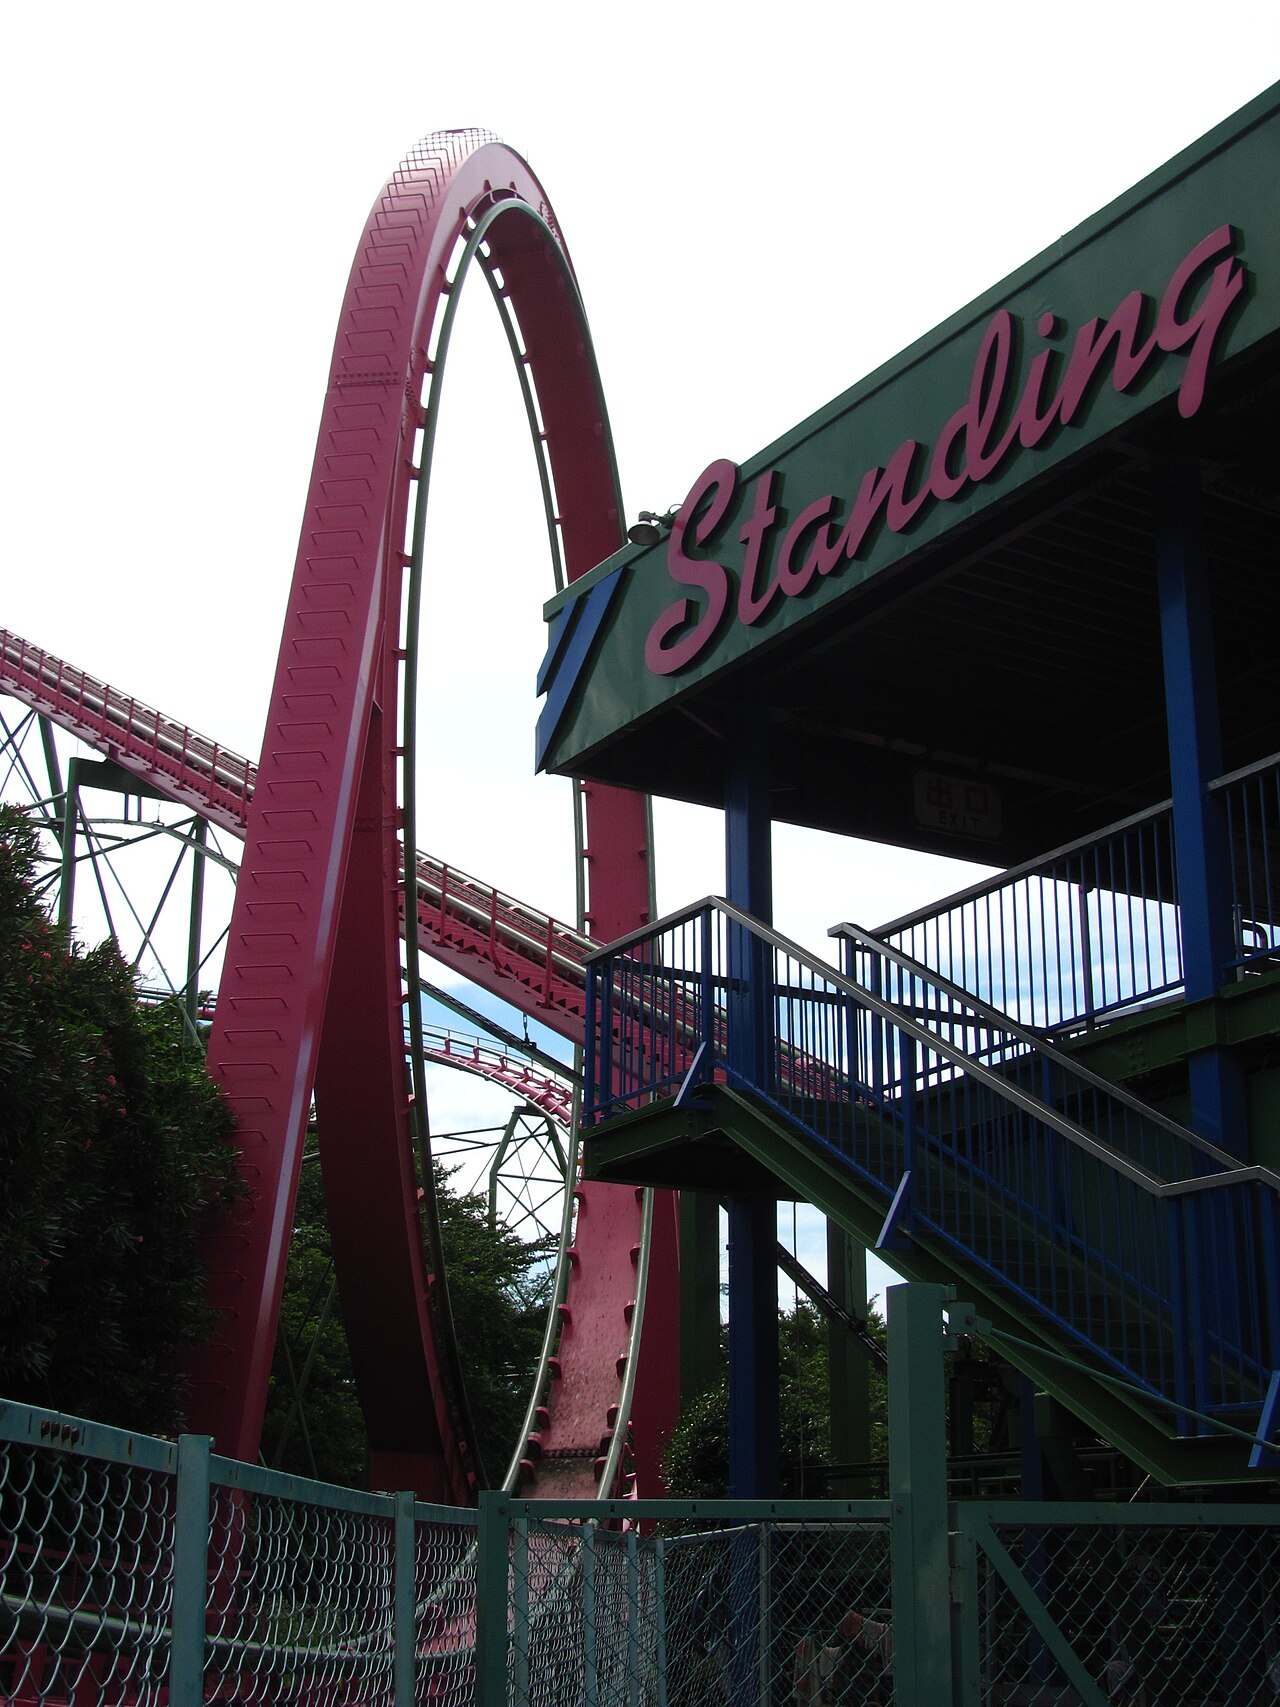
\includegraphics[width=0.38\linewidth]{images/book3/roller-coaster-loop.jpg}

{\small 竖直环形轨道（东京读卖乐园）：轨道为水滴形而非圆形，使曲率在速率最小的顶部最大——这正是周末问题的几何。照片：Jeremy Thompson，CC~BY~2.0。}
\end{omfigure}

\section{问题：过山车环形轨道}

\begin{problem}[{周末问题——汽车以每小时九十千米的速率进入竖直环形轨道：何处减速，
加速度指向何方，乘客感受到多少个 $g$，
以及为何现代环形轨道
不是圆形}]
\label{pb:b1:point-kinematics:1}
一辆汽车视为\omterm{def:b1:point-kinematics:frame}{质点} $M$，沿竖直圆形环轨运动，
环轨半径 $R = \qty{10}{m}$，圆心为 $C$。其位置由
夹角 $\theta$ 确定，它是 $\vect{CM}$ 与竖直向下方向之间的夹角（$\theta =
0$ 对应最低点，$\pi$ 对应最高点）。忽略摩擦，速率规律
（在\cref{ch:b1:work-and-energy}中推导）为
\[
v^2 = v_0^2 - 2gR(1 - \cos\theta),
\]
其中 $v_0 = \qty{25}{m/s}$ 为最低点的速率；$g = \qty{9.81}{m/s^2}$。

\medskip
\noindent\textbf{第一部分——圆周上的运动学。}
\begin{enumerate}
  \item 在以 $C$ 为极点的\omterm{def:b1:point-kinematics:cylindrical}{极坐标}中（$\vect e_r$ 由 $C$
        指向 $M$），写出\omterm{cor:b1:point-kinematics:circular}{圆周运动}的 $\vect v$ 与 $\vect a$。
  \item 求弗勒内矢量 $\vect T$ 和 $\vect N$，
        用 $\vect e_r$ 与 $\vect e_\theta$ 表示，并求\omterm{def:b1:point-kinematics:frenet}{曲率半径}。
  \item 求最高点以及两侧点
        $\theta = \pi/2$ 和 $3\pi/2$ 处的速率。
  \item 对速率规律关于时间求导，证明\omterm{thm:b1:point-kinematics:frenet}{切向加速度}为
        $a_T = -g\sin\theta$，并解释上升与下降
        过程中其符号的含义。
  \item 求\omterm{thm:b1:point-kinematics:frenet}{法向加速度} $a_N(\theta)$ 的表达式，并计算它在
        最低点、两侧与最高点处的值。
  \item 给出四个特征点处 $\vect a$ 的模，以及
        它在最高点处与竖直方向所成的夹角。
  \item 在哪些点上 $\vect a$ 与 $\vect v$ 垂直？哪些点上二者平行？
\end{enumerate}

\medskip
\noindent\textbf{第二部分——角速率与计时。}
\begin{enumerate}[resume]
  \item 将 $\dot\theta$ 表示为 $\theta$ 的函数，并求其
        在最低点与最高点处的值。
  \item 证明 $\ddot\theta = -(g/R)\sin\theta$（即单摆方程），
        并作评论。
  \item 作为比较，求长为 $R$ 的
        单摆做小幅振动的周期（\cref{ex:b1:units-dimensions:pendulum}
        给出了其形式；$k = 2\pi$）。
  \item 利用四个参考点处速率的平均值，估算
        汽车绕环轨一周所需的时间。
  \item 汽车在最高点保持在轨道上的最小速率
        （下一章讨论）为 $\sqrt{gR}$。该条件是否满足？
        所需的最小 $v_0$ 为多少？
\end{enumerate}

\medskip
\noindent\textbf{第三部分——乘客的感受。}
乘客感受到的单位质量视重为 $\vect a - \vect g$
（在本阶段不加证明地承认，推导见\cref{ch:b1:newton-dynamics}）；其以
$g$ 为单位的模称为“$g$ 载荷”。
\begin{enumerate}[resume]
  \item 求最低点处的 $g$ 载荷。
  \item 求最高点处的该载荷，并说明乘客是被压向
        座椅还是约束装置。
  \item 求两侧点处的该载荷。
  \item 乘客短时间内大约能承受 $4g$。该环轨能否通过？
        问题出在何处？
  \item 证明：对于圆形环轨，若进入环轨时的速率恰好
        能够通过最高点（此处视重为零），则最低点的 $g$ 载荷
        必为 $6g$，与 $R$ 无关。
\end{enumerate}

\medskip
\noindent\textbf{第四部分——回旋曲线环轨。}
现代环轨呈“水滴形”：\omterm{def:b1:point-kinematics:frenet}{曲率半径}在最低点处较大，
在最高点处较小。
\begin{enumerate}[resume]
  \item 利用 $\vect a$ 的弗勒内形式，解释沿轨道改变
        $\rho$ 会改变 $a_N$，却不改变速率规律
        （速率规律只依赖于高度）。
  \item 选取 $\rho_{\text{最低点}}$，使最低点处的 $g$ 载荷为
        $3g$，且 $v_0 = \qty{25}{m/s}$。
  \item 最高点仍比最低点高出 $2R = \qty{20}{m}$，
        选取 $\rho_{\text{最高点}}$，使该处的 $g$ 载荷为
        $1.5g$。
  \item 回旋曲线的曲率与弧长成正比，
        $1/\rho = s/A^2$。沿此入口，速率近似不变，
        $a_N$ 随时间如何增长？这样为何比圆形
        （圆形中 $a_N$ 在入口处跳变）对颈部更温和？
  \item 定性地画出所得环轨的形状，并用两句话概括
        它取代圆形环轨的原因。
\end{enumerate}

\medskip
\noindent\textbf{第五部分——从地面观察。}
地面上的一台\omterm{def:b1:optical-instruments:camera}{照相机}，在环轨所在平面内，距环轨中心 \qty{50}{m}，
跟随汽车运动。
\begin{enumerate}[resume]
  \item 当汽车位于最高点、沿水平方向以
        \qty{15}{m/s} 的速率运动时，\omterm{def:b1:optical-instruments:camera}{照相机}需以多大的角速率（rad/s）转动？
        （取\omterm{def:b1:optical-instruments:camera}{照相机}为极点的\omterm{def:b1:point-kinematics:cylindrical}{极坐标}。）
  \item 为何以恒定角速率转动的\omterm{def:b1:optical-instruments:camera}{照相机}不能很好地跟踪
        匀速\omterm{cor:b1:point-kinematics:circular}{圆周运动}？
  \item 概括本章从该环轨中得到的启示：
        哪一种坐标系回答了哪个问题。
\end{enumerate}
\end{problem}
